\documentclass{../template/tp}
\usepackage[utf8x]{inputenc}

\usepackage[english]{babel}
\usepackage[T1]{fontenc}

\usepackage{graphicx}
\usepackage{amssymb}
\usepackage{amsmath}
\usepackage{wasysym} %smiley
\usepackage{hyperref}% hyperliens
\usepackage{tikz}
\usetikzlibrary{babel,positioning,calc}
\usepackage[]{circuitikz}
\usepackage{textcomp}
% \usepackage{minted}
\usepackage[long]{datetime}
\usepackage{gensymb} % \ohm, celsius
\usepackage{framed}
\usepackage{pdfpages}
\usepackage{todonotes}
\usepackage{enumitem}
\usepackage{ marvosym }
\usepackage{qrcode}%Don't forget to escape the "#", as the href package requires.
\usepackage{tabularx}

\usepackage{mathastext} % math as standfard text : units are respecting typography conventions.
\usepackage{fancyhdr}
% \langexam{frenchb}

\usepackage{subcaption}

\graphicspath{{imgs/}}

\newcommand{\labTitle}{Ladder diagrams}
\newcommand{\labNumber}{1}

\newcommand{\version}{v1.0.0}

\newcommand{\mnemonic}{ELEC-H-516}
\newcommand{\courseName}{Programmable Logic Controllers}

\newboolean{koriG}
\ifx\koriG\undefined
\correction{false}
\else
\correction{true}
\fi

% \correction{false}
% \correction{true}

\author{The Fantastic Four}


%% fancy header & foot
\pagestyle{fancy}
\lhead{[\mnemonic] \courseName\\ LABO  \labNumber :  \labTitle}
\rhead{\version\\ page \thepage}
\cfoot{}
%%

\pdfinfo{
/Author (ULB -- BEAMS)
/Title (Labo \labNumber \mnemonic, \labTitle)
/ModDate (D:\pdfdate)

}
\hypersetup{
pdftitle={Labo \labNumber [\mnemonic] \courseName : \labTitle},
pdfauthor={©2017 ULB - BEAMS  },
pdfsubject={\labTitle}
}


\setlength{\parskip}{0.5cm plus4mm minus3mm} %espacement entre §
\setlength{\parindent}{0pt}

\begin{document}

\tptitle{}{Labo \labNumber : \labTitle}

\vspace{-1cm}

\paragraph{Prepartion work}
Spend some time to browse (and read) the ``Basic usage of CoDeSys 3.5'' supplied as pdf. This will help you out figuring out how to use the software. Start with project set-up, Ladder specification, IO specification and simulation.

\rule{\linewidth}{.5pt}

\Question{
	Consider the reservoir system shown on Figure 1. We have water level indicators marked: \texttt{I0.0} and \texttt{I0.1}.
	The sensors indicate 1 when they are fully immersed in the water.
	We want to maintain the level in the reservoir in such a way, so that the water level never goes bellow the level marked with the sensor \texttt{I0.1} (Figure~\ref{fig:reservoir-empty}).
	The level is maintained using a water pump controlled by the variable \texttt{Q0.0}.
	Establish the Ladder diagram of the problem and show the correct operation sequence.
}{}

\Question{
	We will consider rail crossing problem illustrated on Figure~\ref{fig:crossing} (there is only one railway track that can be occupied by only one train at a time).
	Three detectors labeled a, b and c are placed on the rails and are used to control the opening/closing of the barrier.
	When the train passes through a or c, the barrier should close.
	When the train leaves the crossing, \textit{i.e.} when b is released, the barrier should open.
	The train can come from any of the two directions and we will suppose that any maneuver inside the sensor zone is forbidden (train will not do reverse). Distances between different sensors are arbitrary. Trains could be of different lengths, in all 4 combinations are possible. If l is the train length, your control should consider the following lengths: l < ab, bc > l > ab, ac > l > bc > ab, l > ac. Build the model of the control logic required to command the opening/closing of the barrier using LD diagrams. Perform simulations for all train length combinations and show proper command.
	
	\begin{figure}[b]
	\begin{minipage}{.45\textwidth}
		\subcaptionbox{}{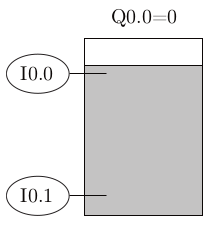
\includegraphics[width=.3\textwidth]{reservoir-full}}
		\subcaptionbox{}{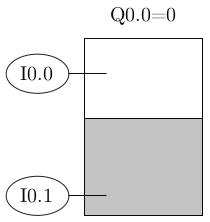
\includegraphics[width=.3\textwidth]{reservoir-mid}}
		\subcaptionbox{\label{fig:reservoir-empty}}{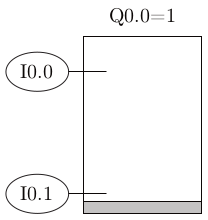
\includegraphics[width=.3\textwidth]{reservoir-empty}}
		\caption{}
	\end{minipage}
	\quad
	\begin{minipage}{.45\textwidth}
		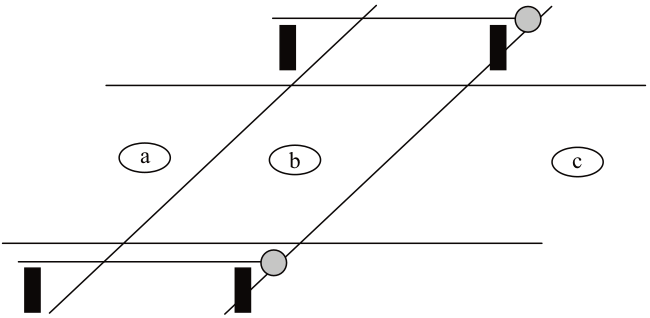
\includegraphics[width=\textwidth]{crossing}
		\caption{}\label{fig:crossing}
	\end{minipage}
	\end{figure}

}{}


\end{document}